\documentclass{article}

\usepackage{tikz}
\usepackage{graphicx} % Required for inserting images

\usepackage[pdftex]{hyperref} 

\usepackage{amsmath}
\usepackage{amssymb}
\usepackage{amsthm}
\newtheorem{theorem}{Theorem}
\newtheorem{proposition}{Proposition}
\newtheorem{lemma}{Lemma}
\newtheorem{corollary}{Corollary}
\theoremstyle{remark}
\newtheorem*{remark}{Remark}

\usepackage{chemfig}
\usepackage[version=4]{mhchem}

\usepackage[style=iso-numeric]{biblatex}
\addbibresource{citations.bib}

\begin{document}

\begin{titlepage}
    \begin{tikzpicture}[remember picture,overlay]
        \node[anchor=north west,yshift=-5mm,xshift=5mm]%
            at (current page.north west)
            {
\includegraphics[height=25mm]{images/EPFL_Logo_Digital_RGB_PROD.png}};
    \end{tikzpicture}
    \begin{center}
        \vspace*{1cm}
            
        \Huge
        \textbf{Exploration of possible structure-based models of the mechanism of action of AAA+ ATPases}
            
        \vspace{0.5cm}
        \LARGE
        %subtitle
            
        \vspace{1.5cm}
            
        \textbf{Antoine Maier - antoine.maier@outlook.com}
            
        \vfill
            
        Master's project for the degree of\\
        Master of Science MSc in Physics
            
        \vspace{0.8cm}
        \Large
        
        Under the supervision of Prof. Paolo De Los Rios\\
        Laboratory of Statistical Biophysics\\
        EPFL\\
        %\today
        February 8, 2024
            
    \end{center}
\end{titlepage}

\tableofcontents
\pagebreak

\section{Introduction}
\label{sec:introduction}
In the general context of cell biology, the study of protein folding is an important topic since their natural tendency to fold into their native conformation is essential for their biological function. This intrinsically stochastic process can lead to misfolding and resulting in amyloids, aggregates of misfolded proteins, which are associated with numerous diseases such as Alzheimer's disease, Parkinson's disease, and type 2 diabetes\cite{chiti_protein_2017}. To prevent this, cells have developed a complex machinery of molecular chaperones to assist the folding of other proteins. Understanding their mechanism of action is essential as it could lead to new therapeutic strategies to treat amyloid-related diseases.

This work focuses on a particular class of molecular chaperones, Hsp100 disaggregases, which belong to the AAA+ ATPase superfamily\cite{tucker_aaa+_2007}. These proteins are typically hexameric oligomers with a central channel through which they translocate substrates\cite{mayer_gymnastics_2010}. This translocation pulls and unfolds misfolded polypeptides out of aggregates that are then dissolved or refolded with the help of other chaperones. However, the mechanism of translocation is still poorly understood, and it is the subject of this work. Shorter J. et al. have proposed a model of the translocation mechanism based on structural biology data, in which a sequential hand-over-hand motion of the protomers is responsible for the translocation\cite{shorter_spiraling_2019}. We will refer to this model as the Sequential Clockwise/2-Residue Step (SC/2R) model. In this work, we propose an alternative model, the Random Protomer Concertina Locomotion (RPCL) model, based on simple physical assumptions about the interaction potential between two neighboring protomers and the resulting minimal energy configuration of the ATPase. We translate these models into the kinetic scheme framework to study the dynamics of the ATPase via simulations and analytical calculations. By comparing the two models with experimental data, we ultimately argue that the RPCL model should be favored over the SC/2R model. The method used is general and could be applied to other translocation models, although this work focuses on the SC/2R and RPCL models.

This document is organized as follows. In Sec.~\ref{sec:theory}, we introduce the kinetic scheme theory, the formulas to compute the quantities of interest, and the simulation algorithm. In Sec.~\ref{sec:models}, we detail the SC/2R and RPCL models and translate them into the kinetic scheme framework. In Sec.~\ref{sec:experiments}, we present some experiments we conducted on the dynamics of the two models: a direct comparison in ideal conditions, the effect of an external force, and the effect of a defective protomer. Finally, in Sec.~\ref{sec:conclusion}, we conclude and discuss some perspectives for future research.


\section{Theory of master equation and kinetic scheme}
\label{sec:theory}
Consider a stochastic system evolving continuously, jumping from one discrete state to another. The state of the system at time $t$ is denoted by the random variable $S(t)=i$, where $i=1,2,\dots,N$, and we assume that the state entirely determines the system, i.e. the trajectory of the system is independent of its history. In other terms, the system is a continuous time Markov chain.
The transitions between the states represent physical or chemical reactions that we assume are all reversible and independent of each other. Each reaction $i\to j$ follows an exponential distribution of rate $k_{ij}$.
The dynamics are the following: the system starts in state $i$ at time $t=0$, sojourns there until one reaction $i\to j$ occurs, and then immediately jumps to state $j$. The system then sojourns in state $j$ until another reaction $j\to k$ occurs, and so on. 

We can represent such a system with a kinetic scheme, a directed graph where each node represents a state, and each reaction $i\to j$ is represented by a directed edge from $i$ to $j$, weighted with the reaction rate $k_{ij}$. We denote the successors and predecessors of a state $i$ by $R_i^+$ and $R_i^-$ respectively. 
We assume that the kinetic scheme is connected. If not, the system would have several independent subsystems that could be studied separately. 

Given the stochastic nature of the system, we are interested in the probability of being in state $j$ at a given time $t$, denoted by $p_j(t):=\mathbb{P}(S(t)=j)$. Its time evolution is given by the $N$ coupled differential master equations:
\begin{equation}
\label{eq:master-equation-kinetic-scheme}
    \dot{p}_j(t) = \sum_{i\in R_j^-}p_i(t)k_{ij} - p_j(t)\sum_{k\in R_j^+}k_{jk} = \sum_{i=1}^N \left(p_i(t)k_{ij} - p_j(t)k_{ji}\right)
\end{equation}
where we used the convention $k_{ii}=0$ for all $i$ and $k_{ij}=0$ if there is no edge from $i$ to $j$ in the kinetic scheme. See App.~\ref{app:master-equation} for a rigorous derivation.
We can rewrite the master equation in matrix form:
\begin{equation}
\label{eq:master-equation-matrix-form}
    \dot{\mathbf{p}}(t) = \mathbf{M}\mathbf{p}(t)
\end{equation}
where $\mathbf{p}(t)$ is the column vector of components $p_i(t)$ and $\mathbf{M}$ is the matrix of components $M_{ij}=k_{ji} - \delta_{ij}\sum_{k=1}^N k_{ik}$, where $\delta_{ij}$ is the Kronecker delta.
With the initial condition $\mathbf{p}(0)$, the solution of Eq~\eqref{eq:master-equation-matrix-form} is:
\begin{equation}
    \mathbf{p}(t) = e^{\mathbf{M}t}\mathbf{p}(0)
\end{equation}

These systems have interesting properties, the most important being the existence and uniqueness of an attracting steady-state distribution $\mathbf{p}^*$, which is in addition globally stable, i.e., any initial condition converges to $\mathbf{p}^*$ as $t\to\infty$, exponentially fast moreover. The properties of such systems are discussed in detail in~\cite{schnakenberg_network_1976}. Still, for mathematical elegance, we give an alternative proof of the existence and uniqueness of the steady-state distribution in App.~\ref{app:steady-state-dist} using almost solely linear algebra. 
To sum up, the stochastic matrix $M$ has rank $N-1$, and thus, the steady-state distribution is given by the unique positive and normalized solution of the linear system:
\begin{equation}
\label{eq:steady-state-dist}
    \mathbf{M}\mathbf{p}^* = \mathbf{0}
\end{equation} 
A convenient way to directly find the steady-state distribution is to note that the sum of the first $N-1$ rows equals minus the last row:
\begin{equation}
    \sum_{i=1}^{N-1} M_{ij} = \sum_{i=1}^{N-1} k_{ji} - (1-\delta_{jN})\sum_{k=1}^N k_{jk} = -k_{jN} + \delta_{jN}\sum_{k=1}^N k_{Nk} = -M_{Nj}
\end{equation}
which means that we can remove the last row without changing the solution of the linear system. Therefore, we modify $\mathbf{M}$ to $\tilde{\mathbf{M}}$ by replacing the last row with ones, and then the steady-state distribution is the unique solution of the linear system:
\begin{equation}
\label{eq:steady-state-tricks}
    \tilde{\mathbf{M}}\mathbf{p}^*
    =
    \begin{pmatrix}
        M_{1,1} & \cdots & M_{1,N} \\ 
        \vdots  & \ddots & \vdots  \\ 
        M_{N-1,1} & \cdots & M_{N-1,N} \\ 
        1 & \cdots & 1
    \end{pmatrix}
    \cdot
    \begin{pmatrix}
        p_1^*\\ 
        \vdots\\ 
        p_{N-1}^*\\ 
        p_N^*
    \end{pmatrix}
    =
    \begin{pmatrix}
        0\\ 
        \vdots\\ 
        0\\ 
        1
    \end{pmatrix}
\end{equation}
since the newly added row constrains the solution to be normalized. This gives a general method to solve any system defined by a master equation, or equivalently a kinetic scheme. However, note that solving Eq~\eqref{eq:steady-state-tricks} does not give a deep understanding of the system. The physical meaning comes after algebraic manipulations of the solution. To the best of the author's knowledge, such manipulations are model-dependent and cannot be generalized.

\subsection{Thermodynamic loops}
    At equilibrium, we postulate that the detailed balance holds, i.e. each elementary process $i\to j$ is in equilibrium with its reverse process $j\to i$. Intuitively, this means that the probability flux from $i$ to $j$ equals the flux from $j$ to $i$. Mathematically, this is expressed by:
    \begin{equation}
        \left.\left(p_i^*k_{ij}\right)\right|_{eq.} = \left.\left(p_j^*k_{ji}\right)\right|_{eq.} 
        \Leftrightarrow \left.\left(\frac{p_i^*k_{ij}}{p_j^*k_{ji}}\right)\right|_{eq.} = 1
    \end{equation}
    for all $i,j$, where $\left.p_i^*\right|_{eq.}$ is the equilibrium probability of being in state $i$, which is the steady-state probability when the system is \emph{isolated}. Being isolated means that there are no external factors pushing the system out of equilibrium, which includes not being in contact with a heat bath, experiencing no applied forces, or receiving no ATP input. When isolated, all the rates $k_{ij}$ are at their equilibrium values $\left.k_{ij}\right|_{eq.}$.
    
    Now consider any closed loop in the equilibrium kinetic scheme, i.e. a sequence of reactions $i_1\to i_2\to\dots\to i_n\to i_1$ where $i_1,\dots,i_n$ are distinct states. By multiplying together each reaction's detailed balance equation in the loop, with the convention $i_{n+1}=i_1$, we obtain:
    \begin{equation}
    \label{eq:thermo-loop-law}
    \begin{split}
        1
        &= \left.\left(\prod_{j=1}^n \frac{p_{i_j}^*k_{i_ji_{j+1}}}{p_{i_{j+1}}^*k_{i_{j+1}i_j}}\right)\right|_{eq.} \\
        &= \left.\left(\frac{\left(\prod_{j=1}^n p_{i_j}^*\right)\left(\prod_{j=1}^n k_{i_ji_{j+1}}\right)}{\left(\prod_{j=1}^n p_{i_{j+1}}^*\right)\left(\prod_{j=1}^n k_{i_{j+1}i_j}\right)}\right)\right|_{eq.} \\
        &= \left.\left(\frac{\prod_{j=1}^n k_{i_ji_{j+1}}}{\prod_{j=1}^n k_{i_{j+1}i_j}}\right)\right|_{eq.}
    \end{split}
    \end{equation}
    i.e. at equilibrium, the product of the reaction rates in a direction of the loop is equal to the product of the reaction rates in the reverse direction. This \emph{thermodynamic loop law} constrains the rates of the reactions in the loop: when all the rates except one are chosen, the last one is fixed by the thermodynamic loop law. Note that this law holds even if the loop is connected to other reactions.

    Going further, when the system is not isolated, its steady-state distribution differs a priori from the equilibrium one. In steady-state, the detailed balance does not hold anymore, and the thermodynamic loop law becomes:
    \begin{equation}
        \frac{\prod_{j=1}^n k_{i_ji_{j+1}}}{\prod_{j=1}^n k_{i_{j+1}i_j}} 
        = \exp\left(\frac{\Delta\mu}{T}\right)
    \end{equation}
    where $\Delta\mu\neq 0$ is a thermodynamic force difference that drives the loop out of equilibrium. Despite this, the thermodynamic loop law Eq.~\eqref{eq:thermo-loop-law} derived at equilibrium remains valid even when the system is not isolated, and in particular it constrains constants of the system since, by definition, they are constants and thus have the same value at- and out-of-equilibrium.
    
    Finally, even though each loop in the kinetic scheme gives a constraint on the rates, they are not necessarily independent. For any basis of the cycle space of the kinetic scheme, each fundamental cycle gives an independent constraint on the rates. The choice of the basis is not unique, but any choice results in the same set of constraints. The number of fundamental cycles inherently depends on the structure of the kinetic scheme, and it must be determined case by case\cite{schnakenberg_network_1976}.

\subsection{Quantities of interest}
\label{subsec:quantities-of-interest}
    Given an initial probability distribution, we know its time evolution and the steady-state distribution to which it converges. However, this distribution only tells us about the probability for the system to be in a given state or, equivalently, a node on the kinetic scheme, but nothing about quantities that change when one or more reactions occur and that are not encompassed in the state description of the system. For example, this could be the substrate translocated length, which is not a state of the system but rather a quantity that changes over time. This section gives general results that will be applied to specific cases later.

    Consider a random variable $X(t)$ representing a quantity that evolves in time. We consider $X$ taking value in $\mathbb{N}$, but the following reasoning can be generalized to other cases. 
    
    In general, computing the exact probability distribution for such a quantity can be complex. However, it is easier to find its master equation and then solve it when possible or use it to compute moments of $X(t)$. The formal derivation is in App.~\ref{app:master-equation} except that, unlike Eq.~\eqref{eq:master-equation-kinetic-scheme}, the transition rates are a prior unknown. If we write $p_x(t):=\mathbb{P}(X(t)=x)$ and $w_{xy}$ the transition rate from $x$ to $y$, using the convention $w_{xx}=0$, the master equation is:
    \begin{equation}
    \label{eq:proba-diff-equ}
        \dot{p}_x(t) = \sum_{y\in\mathbb{N}} p_y(t)w_{yx} - p_x(t)\sum_{y\in\mathbb{N}} w_{xy}
    \end{equation}
    
    Multiplying by $x^k$ and summing over $x$ both sides of Eq.~\eqref{eq:proba-diff-equ}, we find a differential equation for the $k$-th moment of the distribution :
    \begin{equation}
    \label{eq:moment-diff-eq}
    \begin{split}
        \frac{d}{dt}\left\langle X^k(t) \right\rangle 
        &= \sum_{x\in\mathbb{N}} x^k\dot{p}_x(t)
        = \sum_{x,y\in\mathbb{N}} x^k p_y(t) w_{yx} - \sum_{x,y\in\mathbb{N}} x^k p_x(t) w_{xy} \\
        &= \sum_{x,y\in\mathbb{N}} p_y(t) w_{yx} \left(x^k - y^k\right)
    \end{split}
    \end{equation}
    and multiplying by $e^{i\theta x}$ instead, we find a differential equation for the characteristic function $\phi_X(\theta, t):=\left\langle e^{i\theta X(t)}\right\rangle$:
    \begin{equation}
    \label{eq:char-diff-eq}
    \begin{split}
        \frac{\partial}{\partial t}\phi_X(\theta, t) 
        &= \sum_{x\in\mathbb{N}} e^{i\theta x}\dot{p}_x(t)
        = \sum_{x,y\in\mathbb{N}} e^{i\theta x} p_y(t) w_{yx} - \sum_{x,y\in\mathbb{N}} e^{i\theta x} p_x(t) w_{xy} \\
        &= \sum_{x,y\in\mathbb{N}} p_y(t) w_{yx} \left(e^{i\theta x} - e^{i\theta y}\right)
    \end{split}
    \end{equation}
    where we used the properties of dummy variables and the fact that we sum over the same set of values in both sums.
    
    If the transition rates depend solely on the difference, i.e. $w_{xy}=w_{x-y}$, Eqs.~\eqref{eq:moment-diff-eq}~and~\eqref{eq:char-diff-eq} simplify to:
    \begin{equation}
    \label{eq:moment-diff-eq-rates-diff}
        \frac{d}{dt}\left\langle X^k(t) \right\rangle
        = \sum_{x,y\in\mathbb{N}} p_y(t) w_{x-y} \left(x^k - y^k\right)
        = \sum_{x,y\in\mathbb{N}} p_y(t) w_{x} \left((y+x)^k - y^k\right)
    \end{equation}
    and 
    \begin{multline}
    \label{eq:char-diff-equ-simp}
        \frac{\partial}{\partial t}\phi_X(\theta, t) 
        = \sum_{x,y\in\mathbb{N}} p_y(t) w_{x-y} \left(e^{i\theta x} - e^{i\theta y}\right)
        = \sum_{x,y\in\mathbb{N}} p_y(t) w_{x} e^{i\theta y} \left(e^{i\theta x} - 1\right) \\
        = \sum_{y\in\mathbb{N}} p_y(t) e^{i\theta y} \sum_{x\in\mathbb{N}} w_{x} \left(e^{i\theta x} - 1\right)
        = \phi_X(\theta, t) \sum_{x\in\mathbb{N}} w_{x} \left(e^{i\theta x} - 1\right)
    \end{multline}
    where we used the change of variable $x\mapsto x+y$ and the fact that we sum over the whole set $\mathbb{N}$.
    
    We can solve Eq.~\eqref{eq:char-diff-equ-simp} using $\phi_X(0, t)=1$
    \begin{equation}
        \phi_X(\theta, t) = \exp\left(t \sum_{x\in\mathbb{N}} w_{x} \left(e^{i\theta x} - 1\right)\right)
    \end{equation}
    
    and then by inverting the Fourier transform, we obtain the probability distribution
    \begin{multline}
        p_x(t) = \frac{1}{\tau}\int_0^\tau \phi_X(\theta, t) e^{-i\theta x} d\theta \\
        = \frac{e^{-t \sum_{y\in\mathbb{N}} w_{y}}}{\tau}\int_0^\tau \exp\left(t \sum_{y\in\mathbb{N}} w_{y} e^{i\theta y} -i\theta x\right) d\theta
    \end{multline}
    with $\tau:=2\pi$, which can be solved analytically in some cases, but generally using numerical methods.
    
    Next, the mean and standard deviation $\sigma$ of the quantity $X(t)$ are derived from the first and second moments using Eq.~\eqref{eq:moment-diff-eq-rates-diff}:
    \begin{equation}
    \label{eq:first-moment}
        \frac{d}{dt}\left\langle X(t) \right\rangle
        = \sum_{x,y\in\mathbb{N}} p_y(t) w_{x} x
        = \sum_{x\in\mathbb{N}} x w_{x}
        \implies \left\langle X(t) \right\rangle = \left\langle X(0) \right\rangle + t \sum_{x\in\mathbb{N}} x w_{x}
    \end{equation}
    \begin{equation}
    \label{eq:second-moment}
        \frac{d}{dt}\left\langle X^2(t) \right\rangle
        = \sum_{x,y\in\mathbb{N}} p_y(t) w_{x} \left(x^2 + 2xy\right)
        = \sum_{x\in\mathbb{N}} x^2 w_{x} + 2 \left\langle X(t) \right\rangle \underbrace{\sum_{x\in\mathbb{N}} x w_{x}}_{\frac{d}{dt}\left\langle X(t) \right\rangle}
    \end{equation}
    and thus
    \begin{equation}
    \begin{split}
    \label{eq:variance-and-std}
        &\frac{d}{dt}\text{Var}(X(t))
        = \frac{d}{dt}\left\langle X^2(t) \right\rangle - 2 \left\langle X(t) \right\rangle \frac{d}{dt}\left\langle X(t) \right\rangle
        = \sum_{x\in\mathbb{N}} x^2 w_{x} \\
        &\implies \text{Var}(X(t)) = \text{Var}(X(0)) + t \sum_{x\in\mathbb{N}} x^2 w_{x} \\
        &\implies \sigma(t) = \sqrt{\text{Var}(X(0)) + t \sum_{x\in\mathbb{N}} x^2 w_{x}}
    \end{split}
    \end{equation}
    
    If the quantity $X(t)$ changes when a reaction occurs, i.e. when an edge of the kinetic scheme is crossed, we can explicitly compute the transition rates. Consider all the reactions that modify $X(t)$ by $x^*$. Then, the transition rate $w_{x^*}$ is the sum over all such reactions of the probability of being at the initial state of the reaction times its reaction rate. Mathematically, if we denote by $R_{x^*}$ the set of reactions that modify $X(t)$ by $x^*$, we have:
    \begin{equation}
    \label{eq:quantity-transition-rate}
        w_{x^*} = \sum_{i\to j\in R_{x^*}} k_{ij} p_i
    \end{equation}
    
    Finally, from Eqs.~\eqref{eq:first-moment}~and~\eqref{eq:quantity-transition-rate}, the average rate of change of the quantity $X(t)$ is given by:
    \begin{equation}
    \label{eq:quantity-rate-of-change}
        \frac{d}{dt}\left\langle X(t) \right\rangle
        = \sum_{x\in\mathbb{N}} \sum_{i\to j\in R_{x}} x k_{ij} p_i
    \end{equation}
    which is physically intuitive: it is the sum over all the reactions that modify $X(t)$ of the probability of being at the initial state of the reaction times its reaction rate.

\subsection{Simulating trajectories via Gillespie algorithm}
    Generally, the differential equations derived in Sec.~\ref{subsec:quantities-of-interest} cannot be solved analytically, and we must resort to numerical methods. The most straightforward method is to simulate sample trajectories of the system, i.e. the sequence of states visited by the system, and then compute statistics with these trajectories. 
    Moreover, the simulated trajectories can also give us confidence in our numerical implementation by comparing the statistics computed numerically with their analytical value.
    
    The Gillespie algorithm is a method to simulate trajectories for a single particle progressing in time on the kinetic scheme, sojourning in a state until a reaction makes it jump to another state.
    
    Starting in state $i$ at time $t=0$, the sojourn time $T_{ij}$ and the next state $j$ are random variables that satisfy the following derivation. Consider the event \emph{reaction $i\to j^*$ occurs in an infinitesimally small interval $[\tau, \tau+\Delta t]$, and no other reaction occurs in $[0, \tau+\Delta t]$}. It is equivalent to $\{(\tau < T_{ij*} < \tau + \Delta t) \wedge (T_{ij} > \tau + \Delta t \text{, } \forall j\neq j*)\}$. Given that all the reactions are independent and follow an exponential distribution with rate $k_{ij}$, the probability of this event is given by:
    \begin{equation}
    \begin{split}
        &\mathbb{P}\left((\tau < T_{ij*} < \tau + \Delta t) \wedge (T_{ij} > \tau + \Delta t \text{, } \forall j\neq j*)\right) \\
        &= \mathbb{P}(\tau < T_{ij*} < \tau + \Delta t) \prod_{j\neq j*} \mathbb{P}(T_{ij} > \tau + \Delta t) \\
        &= e^{-k_{ij*}\tau} \left(1 - e^{-k_{ij^*}\Delta t}\right) \prod_{j\neq j*} e^{-k_{ij}(\tau + \Delta t)} \\
        &= e^{-\sum_j k_{ij}\tau} k_{ij^*} \Delta t + o(\Delta t)
    \end{split}
    \end{equation}
    In the limit $\Delta t\to 0$, we identify the probability density
    \begin{equation}
        p(i\to j, \tau | i) = k_{ij} e^{-\sum_j k_{ij}\tau} = k_{i} e^{-k_{i}\tau} \frac{k_{ij}}{k_{i}}
    \end{equation}
    where $k_i := \sum_j k_{ij}$ is the total rate of leaving state $i$, and in the last step we multiplied by $\frac{k_i}{k_i}$ which allows us to sample the sojourn time and next state $(\tau, j)$ individually. The first term indicates that the sojourn time $\tau$ before leaving state $i$ follows an exponential distribution, where each reaction rate $k_{ij}$ contributes to the total rate $k_i$. The second term indicates that the next state $j$ is sampled from the successor states of state $i$ with probability proportional to the reaction rate $k_{ij}$.
    
    With these mathematical considerations, we can detail the Gillespie algorithm:
    \begin{enumerate}
        \item We start in a random state; we choose to sample it from the steady-state probabilities associated with each state so that the system is already in steady-state;
        \item The sojourn time is sampled from an exponential distribution with rate \emph{the sum of all the reaction rates leaving the current state};
        \item The next state is sampled from the successor states, with probability proportional to their reaction rates;
        \item We update the time and the state, then jump back to 2.
    \end{enumerate}
    The simulation ends when a stopping criterion is reached, for example, a maximum time or a maximum number of iterations.
    

\section{Translocation models}
\label{sec:models}
To model a translocation mechanism by a kinetic scheme, we first consider the simplest case, an idealized version involving a minimal number of states and transitions in order to capture the essence of the model, and as a second step we add more complexity to take into account more realistic features.

\subsection{ATP/ADP-Protomer exchange model}
\label{subsec:atp-adp-exchange-model}
    Before detailing the translocation models, we explain the source of energy that drives the translocation since, aside from thermal agitation, at equilibrium the AAA+ ATPase on average stands still. In the cell, the [ATP]/[ADP] concentration ratio is maintained at $\sim20-1000$, which is considerably greater than its equilibrium value $\sim10^{-5}$\cite{meyrat_atp_2019}. The ATPases in the cell are in contact with a high concentration of ATP, and thus, as we will see, this favors an ADP-bounded protomer to exchange its nucleotide for an ATP from its environment.

    Consider a volume containing proteins, with ATP and ADP floating around. These nucleotides can bound and unbound from the proteins with rates $k_{on}^T$, $k_{off}^T$ and $k_{on}^D$, $k_{off}^D$, where the superscripts $T$ and $D$ stand for ATP and ADP and the subscripts $on$ and $off$ stand for the binding and unbinding reactions, respectively. Writing $\text{P}\equiv\text{Protein}$, $\text{T}\equiv\text{ATP}$ and $\text{D}\equiv\text{ADP}$, the chemical equation of this process is:
    \begin{equation}
        \ce{PT + D <=>[k_{off}^T][k_{on}^T] P + T + D <=>[k_{on}^D][k_{off}^D] PD + T}
    \end{equation}
    Using a simple bimolecular binding/unbinding model for the protein-nucleotide interactions, the corresponding master equations for the concentrations $[.]$ are:
    \begin{equation}
    \begin{split}
        \frac{d[\text{PT}]}{dt} &= k_{on}^T [\text{P}][\text{T}] - k_{off}^T [\text{PT}] \\
        \frac{d[\text{PD}]}{dt} &= k_{on}^D [\text{P}][\text{D}] - k_{off}^D [\text{PD}] \\
        \frac{d[\text{P}]}{dt} &= k_{off}^T [\text{PT}] + k_{off}^D [\text{PD}] - (k_{on}^T + k_{on}^D) [\text{P}]
    \end{split}
    \end{equation}
    We omitted the equations for ATP and ADP concentration evolution because they are redundant in steady-state, which is the state we are ultimately interested in. 
    
    We assume that the sojourn time of the protein not bound to any nucleotide is much shorter than the binding/unbinding times so that we can set $\dot{[\text{P}]}=0$ and thus $[\text{P}]=\frac{k_{off}^T [\text{PT}] + k_{off}^D [\text{PD}]}{k_{on}^T + k_{on}^D}$. Plugging this expression into the bounded complexes equations above and developing the result, we obtain:
    \begin{equation}
        \frac{d[\text{PT}]}{dt} = 
            \underbrace{\frac{k_{off}^D k_{on}^T [\text{T}]}{k_{on}^T [\text{T}] + k_{on}^D [\text{D}]}}_{=:k_{DT}} [\text{PD}]
            - \underbrace{\frac{k_{off}^T k_{on}^D [\text{D}]}{k_{on}^T [\text{T}] + k_{on}^D [\text{D}]}}_{=:k_{TD}} [\text{PT}]
    \end{equation}
    and a similar equation for $[\text{PD}]$ but with opposite signs, where we defined effective exchange rates $k_{DT}$ and $k_{TD}$ for $\text{ADP}\to\text{ATP}$ and $\text{ATP}\to\text{ADP}$ exchange, respectively. This means that under the assumption that the protein spends most of its time bound to a nucleotide, we can rewrite the ATP/ADP exchange as a single reaction:
    \begin{equation}
        \ce{PT <=>[k_{TD}][k_{DT}] PD}
    \end{equation}
    
    One important thing here is that these effective exchange rates depend on the [ATP]/[ADP] concentration ratio, and thus, a direction is favored when it deviates from its equilibrium value. In particular, looking at the ratio of rates
    \begin{equation}
    \label{eq:kdt-ktd-ratio}
        \frac{k_{DT}}{k_{TD}} 
        = \frac{k_{off}^D k_{on}^T}{k_{off}^T k_{on}^D} \frac{[T]}{[D]}
        = \frac{K_d^D}{K_d^T} \frac{[T]}{[D]}
    \end{equation}
    where $K_d^N:=\frac{k_{off}^N}{k_{on}^N}$ is the dissociation constant of the nucleotide $N$, we see that when [ATP]/[ADP] is extraordinarily higher than its equilibrium value, as it is the case in cells, a protein in ADP-bound state is strongly favored to exchange its nucleotide for an ATP from its environment. This is the source that drives the translocation models.
    
    A last important relation is the following. Consider the ratio of the effective exchange rates at equilibrium:
    \begin{multline}
    \label{eq:equil-kdt-ktd-ratio}
        \left.\frac{k_{DT}}{k_{TD}}\right|_{eq.}
        = \frac{K_d^D}{K_d^T} \left.\frac{[T]}{[D]}\right|_{eq.}
        = \frac{K_d^D}{K_d^T} \frac{[T]}{[D]} \frac{[D]}{[T]} \left.\frac{[T]}{[D]}\right|_{eq.} \\
        = \frac{k_{DT}}{k_{TD}} \left(\left.\frac{[T]}{[D]}\right|_{eq.} \middle/ \frac{[T]}{[D]}\right)
    \end{multline}
    This is particularly useful for a thermodynamic loop law Eq~\eqref{eq:thermo-loop-law} involving nucleotide exchange to make [ATP]/[ADP] appear explicitly.

\subsection{Common features of the translocation models}
    Before defining the translocation models themselves, we first detail the common features of these models. The AAA+ ATPase is made of $N$ protomers, $N=6$ for Hsp104, but the models we study can be extended to an arbitrary number of protomers. Each protomer is either in ATP-bound state or in ADP-bound state. Nucleotide-bound state can change due to ATP hydrolysis, with rate $k_h$, spontaneous ATP synthesis, with rate $k_s$, or nucleotide exchange with rates $k_{DT}$ and $k_{TD}$ as detailed in Sec.~\ref{subsec:atp-adp-exchange-model}.

    The substrate translocation mechanism of the ATPase is due to the individual translocation of protomers in a cyclic manner. There are two quantities of interest: the substrate translocated length and the ATP consumption, or similarly, the translocation velocity and ATP consumption rate. The two quantities are measured during simulations and compared to their analytical expected value computed using Eq~\eqref{eq:quantity-rate-of-change}. In both models, the ATPase consumes one ATP molecule and translocates the substrate by $\Delta x$ residues per cycle, where $\Delta x$ depends on the model. In their kinetic scheme, only one transition consumes ATP and only one transition induces a substrate translocation.

    Finally, with the exception of [ATP]/[ADP] for which its equilibrium and in vivo value are known\cite{meyrat_atp_2019}, in the absence of measurements, all the other physical parameters are freely set to a value with order of magnitude $\sim10^{-1}-10^1$.

\subsection{Sequential Clockwise/2-Residue Step (SC/2R) model}
\label{subsec:sc2r-model}
    The exact mechanism of action of substrate translocation of the AAA+ ATPases is far from understood. Shorter J. et al. proposed a hand-over-hand model based on Hsp104 cryoelectron microscopy imaging\cite{shorter_spiraling_2019}. Orienting the Hsp104 such that the amyloid is in the upward direction, its $N=6$ protomers are in a staircase-like configuration. The lowest protomer hydrolyzes its ATP molecule, then translocates upward, parallel to the substrate strand, then stops forming a new stair tread two residues higher than its, previously topmost, left neighbor, and then it exchanges its ADP molecule for an ATP from the bulk. The reaction sequence repeats with the right neighboring protomer, previously the second lowest now the lowest, to hydrolyze its ATP, translocate upwards, exchange its ADP for an ATP, and so on. We call this model Sequential Clockwise/2-Residue Step (SC/2R). Its dynamics are illustrated in a video accessible at \url{https://youtu.be/pqPL35mMfj0}; note that the animator\footnote{Rohaan Waqas (@rohaanwaqas05 on Fiverr)} exercised some creative freedom in its depiction.

    We identify a cycle consisting of three states:
    \begin{itemize}
        \item (A) All protomers are in ATP-bound state;
        \item (B) The lowest protomer is in ADP-bound state, and the others are in ATP-bound state;
        \item (C) The highest protomer (previously the lowest) is in ADP-bound state, and the others are in ATP-bound state.
    \end{itemize}
    We associate the steady-state probability $p_A, p_B, p_C$ to each state A, B, and C.
    The transitions between the states are the following:
    \begin{itemize}
        \item $A\to B$: the lowest protomer hydrolyses its ATP molecule with rate $k_h$ (reverse reaction is spontaneous ATP synthesis with rate $k_s$), which consumes (respectively produces) an ATP molecule;
        \item $B\to C$: the lowest protomer (now in ADP-bound state) translocates upward with rate $k_\uparrow$ (reverse reaction is translocating downward with rate $k_\downarrow$), which translocates the substrate by $\Delta x=2$ (respectively $\Delta x=-2$) residues;
        \item $C\to A$: the highest protomer (previously the lowest) exchanges its ADP molecule with an ATP molecule from the bulk with rate $k_{DT}$ (reverse reaction is ATP $\to$ ADP exchange with rate $k_{TD}$). This exchange process is detailed in Sec.~\ref{subsec:atp-adp-exchange-model}.
    \end{itemize}
    The corresponding kinetic scheme is:
    \vspace*{0.5cm}
    \begin{center}
        \schemestart
            C
            \arrow(TTD--TTT){<->>[$k_{TD}$][$k_{DT}$]}[180,1.1]
            A
            \arrow(@TTT--DTT){<->>[*0 $k_h$][*0 $k_s$]}[-90,1.1] 
            B
            \arrow(@DTT--@TTD){<->>[*0 $k_\uparrow$][*0 $k_\downarrow$]}
        \schemestop
    \end{center}
    \vspace*{0.5cm}
    
    One could argue that more states are needed since different protomers undergo the hydrolysis-translocation-exchange sequence, but the protomers are a priori indistinguishable, and thus, we merge all states that satisfy the state descriptions above. This assumption is lightly discussed in App.~\ref{app:non-ideal-model}.

    The only non-constant rates are the effective exchange rates $k_{DT}$ and $k_{TD}$, which depend on the [ATP]/[ADP] concentration ratio. Obviously, there is a single fundamental cycle in the kinetic scheme, giving us the thermodynamic loop law (Eq.~\eqref{eq:thermo-loop-law}):
    \begin{equation}
    \label{eq:sc2r-thermo-loop-law}
        \frac{k_h k_\uparrow \left.k_{DT}\right|_{eq.}}{k_s k_\downarrow \left.k_{TD}\right|_{eq.}} = 1
    \end{equation}
    We set an arbitrary value for $k_\uparrow$, thus $k_\downarrow$ is constrained by the thermodynamic loop law. 
    
    Solving the linear system Eq.~\eqref{eq:steady-state-dist} for this model, we find the steady-state probabilities:
    \begin{equation}
    \label{eq:sc2r-steady-state-probabilities}
    \begin{split}
        p_A &\propto k_s k_{DT} + k_\downarrow k_s + k_\uparrow k_{DT} \\
        p_B &\propto k_h k_\downarrow + k_{DT} k_h + k_{TD} k_\downarrow \\
        p_C &\propto k_\uparrow k_{TD} + k_s k_{TD} + k_h k_\uparrow
    \end{split}
    \end{equation}
    where the proportionality constant is fixed by the normalization condition $p_A+p_B+p_C=1$. We see that for each state, its steady-state probability is the product of the two rates directly leading to the state, plus the sum of the product or rates of all paths of size 2 leading to the state.
    
    Finally, using Eq.~\eqref{eq:quantity-rate-of-change}, the average velocity $\left\langle v \right\rangle$ and ATP consumption rate $r_{ATP}$ are:
    \begin{equation}
    \begin{split}
        \left\langle v \right\rangle &= \Delta x p_B k_\uparrow - \Delta x p_C k_\downarrow 
            \propto \Delta x \left(k_h k_\uparrow k_{DT} - k_s k_\downarrow k_{TD}\right) \\
        r_{ATP} &= p_A k_h - p_B k_s
            \propto k_h k_\uparrow k_{DT} - k_s k_\downarrow k_{TD}
    \end{split}
    \end{equation}
    where the proportionality constant is the same as the steady-state probabilities Eq~\eqref{eq:sc2r-steady-state-probabilities}. We see that the average velocity and ATP consumption rate are proportional to each other, which is intuitive since in a single loop, all net probability fluxes must be equal by Kirchhoff's law. Moreover, the flux is the product of the rates in one direction of the loop minus the product of the rates in the other direction of the loop. Using the thermodynamic loop law Eq.~\eqref{eq:sc2r-thermo-loop-law}, as well as Eq.~\eqref{eq:equil-kdt-ktd-ratio}, we can rewrite the average velocity as:
    \begin{equation}
    \label{eq:sc2r-average-velocity}
        \left\langle v \right\rangle \propto \Delta x \left(1 - \left.\frac{[T]}{[D]}\right|_{eq.}\bigg/\frac{[T]}{[D]}\right) k_h k_\uparrow k_{DT}
    \end{equation}
    which shows explicitly that the average velocity is directly proportional to the deviation of [ATP]/[ADP] from equilibrium, the product of rates in the main direction of the loop, and the absolute substrate translocation steplength $\Delta x$. This is a general result that holds for any kinetic scheme made of a single fundamental cycle, and it is illustrated numerically in App.~\ref{app:average-velocity-vs-atp-adp-ratio}. 
    
    Finally, we compute the net ATP consumed per translocated residue:
    \begin{equation}
    \label{eq:sc2r-atp-per-residue}
        \frac{\#\text{ATP}}{\#\text{residue}} = \frac{r_{ATP}}{\left\langle v \right\rangle} = \frac{1}{\Delta x} = 0.5
    \end{equation}

\subsection{Random Protomer Concertina Locomotion (RPCL) model}
\label{subsec:rpcl-model}
    Some implications from the SC/2R model do not match experimental data; we will detail this more later. This motivated us to propose a new model, the Random Protomer Concertina Locomotion (RPCL) model.

    This alternative model is based on a simple physical assumption: the height difference of two neighboring protomers is subject to a linear restoring force. We further assume that the spring constant depends only on the nucleotide-bound state of the pair of protomers, and in particular, it is weaker between an ADP-bound and an ATP-bound protomer, than between two ATP-bound protomers. Then, the AAA+ ATPase adopts the minimum energy configuration, which we derive depending on the nucleotide-bound state of its $N$ protomers.

    Let $h_i$ be the height difference between protomer $i+1$ and $i$ and $h_0$ their equilibrium height difference (we choose arbitrarily that protomer $i+1$ is the right neighbor of protomer $i$). We write $k$, the spring constant between two neighboring ATP-bound protomers, and $k'$, the spring constant between an ADP-bound protomer and its right (ATP-bound) neighbors (this choice is explained later). Then, there are in total $N$ interactions (since the protomers are cyclically arranged), and to each restoring force is associated a potential energy $\frac{1}{2}k h_i^2$. The height differences $h_i$ are signed thus they must always sum to zero. 
    
    Let's first find the minimum energy configuration in the case where a single protomer, the $N$-th without loss of generality, is in ADP-bound state, and all the others are in ATP-bound state. The Lagrangian of the system is:
    \begin{equation}
        \mathcal{L} = \frac{1}{2}k \sum_{i=1}^{N-1} (h_i - h_0)^2 + \frac{1}{2}k' (h_N - h_0)^2 - \lambda \sum_{i=1}^N h_i
    \end{equation}
    where $\lambda$ is the Lagrange multiplier associated with the constraint $\sum_{i=1}^N h_i = 0$. Solving the system of equations $\left\{\frac{\partial\mathcal{L}}{\partial h_i}=0 \quad \forall i, \quad \frac{\partial\mathcal{L}}{\partial \lambda}=0\right\}$, we find the minimal energy configuration:
    \begin{equation}
    \begin{cases}
        h_{i\neq N} = h_0 \frac{k-k'}{(N-1)k'+k}, & \\
        h_N = (N-1) h_0 \frac{k'-k}{(N-1)k'+k} = -(N-1) h_{i\neq N} &
    \end{cases}
    \end{equation}
    This is the description of a staircase-like configuration, similar to SC/2R model, where each protomer is $\Delta h := h_{i\neq N}$ higher than its left neighbor, except for the ADP-bound protomer where its weaker interaction $k'<k$ induces a large step down. If we set $\Delta h = 2$ residues, this configuration is identical to SC/2R's configuration. 
    
    When all protomers are in ATP-bound state, the weaker spring constant becomes $k'\mapsto k$, and it results in a flat minimal energy configuration, where $h_i = 0, \: \forall i$. This configuration predicted by RPCL but absent from SC/2R resembles Hsp104's \emph{closed state} experimentally observed\cite{shorter_spiraling_2019}. 
    
    Based on these two configurations, we propose the following dynamics. The ATPase starts in a flat configuration. All the protomers compete independently in parallel to hydrolyze their ATP molecule. The first one to do so prohibits other protomer's hydrolysis and this alters the potential with its right neighbor. Then the ATPase adopts the minimal energy staircase-like configuration, with the right neighbor of the ADP-state protomer fixed to the substrate, by translocating all the other protomers upward, $\Delta h = 2$ residues higher than their left neighbor. With these choices, the protomer that moves the most is the ADP-bound one, somewhat similar to SC/2R, where it was motivated by a cryo-EM measurement, the lower-resolution density being an indicator of conformational flexibility\cite{shorter_spiraling_2019}. Now the ADP-bound protomer exchanges its nucleotide for an ATP from the bulk, which induces the ATPase to contract upward, back to the flat configuration. For this transition, we propose that it's the previously ADP-bound protomer that stays fixed to the substrate and all other protomers that translocate upwards. This cycle repeats, and the substrate is translocated by $\Delta x = (N-1)\Delta h = 10$ residues per cycle. The name \emph{concertina locomotion} takes its inspiration from a type of locomotion that some snakes use to climb trees.\footnote{See \url{https://en.wikipedia.org/wiki/Concertina_movement\#Modes\#Arboreal}} Its dynamics are illustrated in a video accessible at \url{https://youtu.be/95A3J68zQ0Q}; note that the animator\footnote{Rohaan Waqas (@rohaanwaqas05 on Fiverr)} exercised some creative freedom in its depiction.
    
    To transpose this model in the kinetic scheme framework, we identify 4 states in the cycle:
    \begin{itemize}
        \item (A) All protomers are in ATP-bound state and the ATPase is in a flat configuration;
        \item (B) A single randomly chosen protomer is in ADP-bound state and the ATPase is in a flat configuration;
        \item (C) The ATPase is in a staircase-like configuration with the ADP-bound protomer being the highest one;
        \item (D) All protomers are in ATP-bound state, and the ATPase is in a staircase-like configuration.
    \end{itemize}
    We associate to each state A, B, C, D the steady-state probability $p_A, p_B, p_C, p_D$, respectively. 
    
    Again merging all the indistinguishable states (assumption lightly discussed in App.~\ref{app:non-ideal-model}), the transitions between the states are the following:
    \begin{itemize}
        \item $A\to B$: a random protomer hydrolyses its ATP molecule with rate $k_h$ (reverse reaction is spontaneous ATP synthesis with rate $k_s$), which consumes (respectively produces) an ATP molecule. But since there are $N$ protomers, and each protomer is equally likely to hydrolyze its ATP molecule, in the kinetic scheme this reaction has an effective rate $\bar{k}_h = N k_h$. The reverse reaction is left unchanged;
        \item $B\to C$: the ATPase extends upward, the right neighbor of ADP-bound protomer being fixed and all other protomers stop $\Delta h = 2$ residues higher than their left neighbor, to adopt the staircase-like configuration with rate $k_{\uparrow ext.}$ (reverse reaction is to contract downward with rate $k_{\downarrow cont.}$), which induces a substrate translocation of $\Delta x=2(N-1)=10$ (respectively $\Delta x=-2(N-1)=-10$) residues;
        \item $C\to D$: the previously ADP-bound protomer exchanges its ADP molecule with an ATP molecule from the bulk with rate $k_{DT}$ (reverse reaction is ATP $\to$ ADP exchange with rate $k_{TD}$). This exchange process is detailed in Sec.~\ref{subsec:atp-adp-exchange-model};
        \item $D\to A$: the ATPase contracts upward, the previously ADP-bound protomer being fixed to the substrate, all the other protomers translocate upward, to adopt the flat configuration with rate $k_{\uparrow cont.}$. This is not considered substrate translocation because we choose arbitrarily the height of the topmost protomer to be the reference when measuring substrate translocation. The reverse reaction is to extend downward with rate $k_{\downarrow ext.}$ for a single protomer, but since in the full-ATP-flat configuration this reaction could be induced by any of the $N$ protomers, in the kinetic scheme we associate to this reaction an effective rate $\bar{k}_{\downarrow ext.}=Nk_{\downarrow ext.}$.
    \end{itemize}
    The kinetic scheme of this model is
    \vspace*{0.5cm}
    \begin{center}
        \schemestart
        A
        \arrow(FlatT--FlatD){<->>[*0 $\bar{k}_h$][*0 $k_s$]}[-90,1.1] 
        B
        \arrow(@FlatD--ExtendedD){<->>[$k_{\uparrow ext.}$][$k_{\downarrow cont.}$]}[,1.1]
        C
        \arrow(@ExtendedD--ExtendedT){<->>[*0 $k_{DT}$][*0 $k_{TD}$]}[90,1.1]
        D
        \arrow(@FlatT--@ExtendedT){<<->[$\bar{k}_{\downarrow ext.}$][$k_{\uparrow cont.}$]}[,1.1]
    \schemestop
    \end{center}
    \vspace*{0.5cm}
    
    Similarly to the SC/2R model, only effective exchange rates $k_{DT}$ and $k_{TD}$ are non-constants and depend on the [ATP]/[ADP] concentration ratio. All the protomer translocation rates are freely set, except for $k_{\downarrow cont.}$ which is constrained by the thermodynamic loop law (Eq.~\eqref{eq:thermo-loop-law}):
    \begin{equation}
    \label{eq:rpcl-thermo-loop-law}
        \frac{k_h k_{\uparrow ext.} \left.k_{DT}\right|_{eq.} k_{\uparrow cont.}}{k_s k_{\downarrow cont.} \left.k_{TD}\right|_{eq.} k_{\downarrow ext.}} = 1
    \end{equation}
    It is irrelevant to use the bar constants in the thermodynamic loop law or not since they appear in the numerator and the denominator, and thus cancel out.
    
    We then solve the linear system Eq.~\eqref{eq:steady-state-dist} for this system to obtain the steady-state probabilities:
    \begin{equation}
    \label{eq:rpcl-steady-state-probabilities}
    \begin{split}
        p_A &\propto k_s k_{\downarrow cont.} k_{\uparrow cont.} + k_s k_{DT} k_{\uparrow cont.} + k_s k_{\downarrow cont.} k_{TD} + k_{\uparrow ext.} k_{DT} k_{\uparrow cont.} \\
        p_B &\propto \bar{k}_h k_{\downarrow cont.} k_{TD} + \bar{k}_h k_{\downarrow cont.} k_{\uparrow cont.} + k_{\downarrow cont.} k_{TD} \bar{k}_{\downarrow ext.} + \bar{k}_h k_{DT} k_{\uparrow cont.} \\
        p_C &\propto k_{\uparrow ext.} k_{TD} \bar{k}_{\downarrow ext.} + \bar{k}_h k_{\uparrow ext.} k_{TD} + k_s k_{TD} k_{\downarrow ext.} + \bar{k}_h k_{\uparrow ext.} k_{\uparrow cont.} \\
        p_D &\propto k_s k_{DT} \bar{k}_{\downarrow ext.} + k_{\uparrow ext.} k_{DT} \bar{k}_{\downarrow ext.} + k_s k_{\downarrow cont.} \bar{k}_{\downarrow ext.} + \bar{k}_h k_{\uparrow ext.} k_{DT}
    \end{split}
    \end{equation}
    where the proportionality constant is fixed by the normalization condition $p_A+p_B+p_C+p_D=1$. We see that for each state, its steady-state probability is the sum of the product of rates of all combinations of paths of size 1 and 2 leading to the state, plus the sum of the product of rates of all paths of size 3 leading to the state.
    
    Similarly to the SC/2R model, we compute the average velocity $\left\langle v \right\rangle$ and express it as a function of the concentration ratio, the ATP consumption rate $r_{ATP}$, and the net ATP consumed per translocated residue:
    \begin{equation}
    \label{eq:rpcl-quantities-of-interest}
    \begin{split}
        &\begin{split}
            \left\langle v \right\rangle 
            &\propto \Delta x \left(\bar{k}_h k_{\uparrow ext.} k_{DT} k_{\uparrow cont.} - k_s k_{\downarrow cont.} k_{TD} \bar{k}_{\downarrow ext.}\right) \\
            &\propto \Delta x \left(1 - \left.\frac{[T]}{[D]}\right|_{eq.}\bigg/\frac{[T]}{[D]}\right) \bar{k}_h k_{\uparrow ext.} k_{DT} k_{\uparrow cont.}
        \end{split} \\
        &r_{ATP} \propto \bar{k}_h k_{\uparrow ext.} k_{DT} k_{\uparrow cont.} - k_s k_{\downarrow cont.} k_{TD} \bar{k}_{\downarrow ext.} \\
        &\frac{\#\text{ATP}}{\#\text{residue}} = \frac{r_{ATP}}{\left\langle v \right\rangle} = \frac{1}{\Delta x} = 0.1
    \end{split}
    \end{equation}
    where the proportionality constant is the same as the steady-state probabilities Eq.~\ref{eq:rpcl-steady-state-probabilities}. All the conclusions of the SC/2R model due to being made of a single fundamental cycle hold for the RPCL model as well, with the difference that the ATP consumed per translocated residue is five times smaller.
    
    

\section{Experiments}
\label{sec:experiments}
This section presents some experiments on the SC/2R and RPCL models to highlight their similarities and differences. The results are compared to experimental data when available. The code used to generate these results is available at \url{https://github.com/antmaier/Projet-de-Master.git}.

\subsection{Dynamics comparison}
    We begin by simulating some trajectories of the two models under ideal conditions and compute some statistics. In Fig.~\ref{fig:trajectories}, we show some sample trajectories of the two models in solid colored lines, the analytical expected substrate translocation and standard deviation using Eqs.~\eqref{eq:first-moment}~and~\eqref{eq:variance-and-std} in grey solid line and pale colored areas, the empirical standard deviation in dashed lines, and the ATP consumption per translocated residue. We plot as well the distribution of sojourn times between translocation events.

    To compare the two models, their rates are scaled by a factor so that their analytical average velocity is normalized. The constants' exact values are irrelevant; the essential point is that [ATP]/[ADP] concentration ratio is set to a large value similar to in vivo conditions, and its equilibrium value very small, which results in a non-zero average substrate translocation velocity of the AAA+ ATPase. All the other free parameters are set to values of the order of 1 before renormalization.

    \begin{figure}[h]
    \centering
    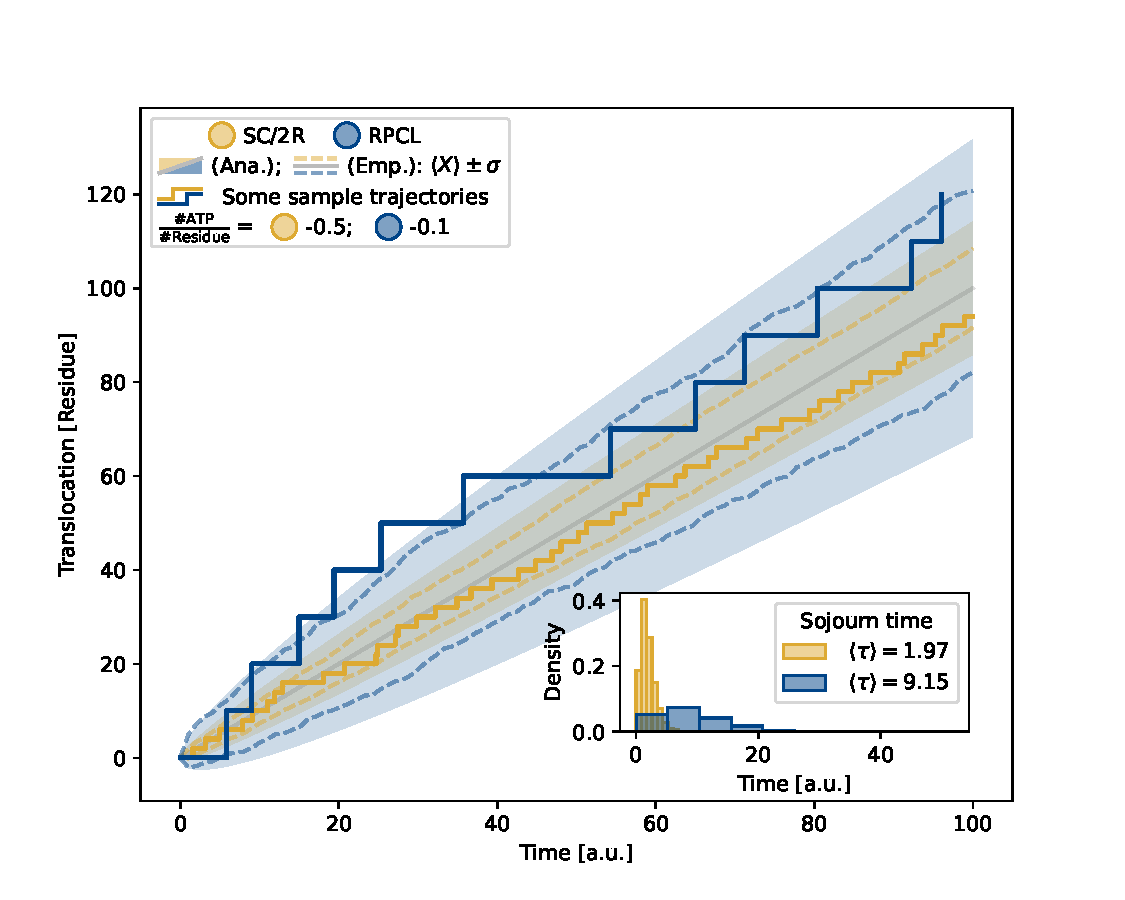
\includegraphics[width=\textwidth]{images/trajectories.pdf}
    \caption{Trajectories and statistical analyses comparing SC/2R (yellow) and RPCL (blue) models of AAA+ ATPase substrate translocation mechanism. Solid colored lines represent sample trajectories for each model, grey solid line and pale areas depict analytical expected substrate translocation and standard deviation, and dashed lines show empirical standard deviation. Empirical ATP consumption per translocated residue and distribution of sojourn times between translocation events are computed. Physical rates are scaled for normalized average velocity, with constants adjusted to maintain ATPase activity.}
    \label{fig:trajectories}
    \end{figure}
    
    As predicted by the calculations in Secs.~\ref{subsec:sc2r-model}~and~\ref{subsec:rpcl-model}, RPCL consumes five times less ATP than SC/2R for a similar average velocity, due to substrate translocation steplength and sojourn time five times longer consuming a single ATP molecule, as visible on the sample trajectories and sojourn times histograms. RPCL dynamics are more consistent with experimental data where it has been shown that the ATPase moves by steps of $14.6\pm 0.9$ amino acids for single-strand translocation\cite{avellaneda_processive_2020}, the setup we simulate in this work.
    
    One behavior that we fail to understand is the discrepancy between analytical and numerical standard deviations. With a convergence analysis, we have ruled out the hypothesis of a sampling error. We suspect that our analytical expression Eq.~\eqref{eq:variance-and-std}) is incorrect, but this issue has not yet been resolved.

\subsection{Adding an external force}
\label{subsec:force}
    Now, we investigate how the dynamics are modified in the presence of an external constant force pulling on the substrate, opposing the AAA+ ATPase translocation. The force thus derives from a potential energy $U(x) \propto x$, where $x$ is the substrate translocated length, and we fix $u$ the potential energy for a unit translocation $\Delta x = 1$ residue. Following the Arrhenius law, the presence of this potential modifies the rate of reactions that induce a substrate translocation $\Delta x$ by $k\mapsto k e^{-\beta u \Delta x }$, where $\beta$ is the inverse temperature, and we assume that the pre-exponential factor is already contained in the rate $k$. This additional Boltzmann factor does not influence the thermodynamic loop law Eq.~\eqref{eq:thermo-loop-law} since at equilibrium, the force is zero, the potential energy is constant, and thus for any reaction that induces a substrate translocation $\Delta x$, the Boltzmann factor equals one. Therefore, a rate constrained by the loop law is similarly modified, i.e. $k\mapsto k e^{-\beta u \Delta x }$, where $k$ is the constrained rate. However, the additional term does influence the dynamics for non-zero forces. Physical quantities are computed by replacing old rates with new ones containing the Boltzmann factor.

    In practical terms, both SC/2R and RPCL models are made of a single loop with a single reaction associated with a translocation of the substrate. Thus, after fixing an arbitrary value $u/T$, the rates are transformed as follows:
    \begin{itemize}
        \item $k_\uparrow\mapsto k_\uparrow e^{-2 \frac{u}{T}}$ and $k_\downarrow\mapsto k_\downarrow e^{2 \frac{u}{T}}$ for SC/2R;
        \item $k_{\uparrow ext.} \mapsto k_{\uparrow ext.} e^{-10 \frac{u}{T}}$ and $k_{\downarrow cont.} \mapsto k_{\downarrow cont.} e^{10 \frac{u}{T}}$ for RPCL.
    \end{itemize}
    
    In Fig.~\ref{fig:force}, we show the average velocity as a function of the thermally scaled unit potential energy $u/T$ for both models. It is irrelevant to compare their numerical values here since their rates are set arbitrarily and do not necessarily correspond to the same physical quantities. The key point is the qualitative behavior of the average velocity as a function of the force, which we can see is similar for both models. In particular, we see that the average velocity is modified as soon as we apply a non-zero force. This is an argument in disfavor of the experimental result where the velocity is unaffected by the force up to a threshold value, after which the velocity drastically falls\cite{avellaneda_processive_2020}. However, this result must be taken cautiously due to their high measurement uncertainties.

    \begin{figure}[h]
        \centering
        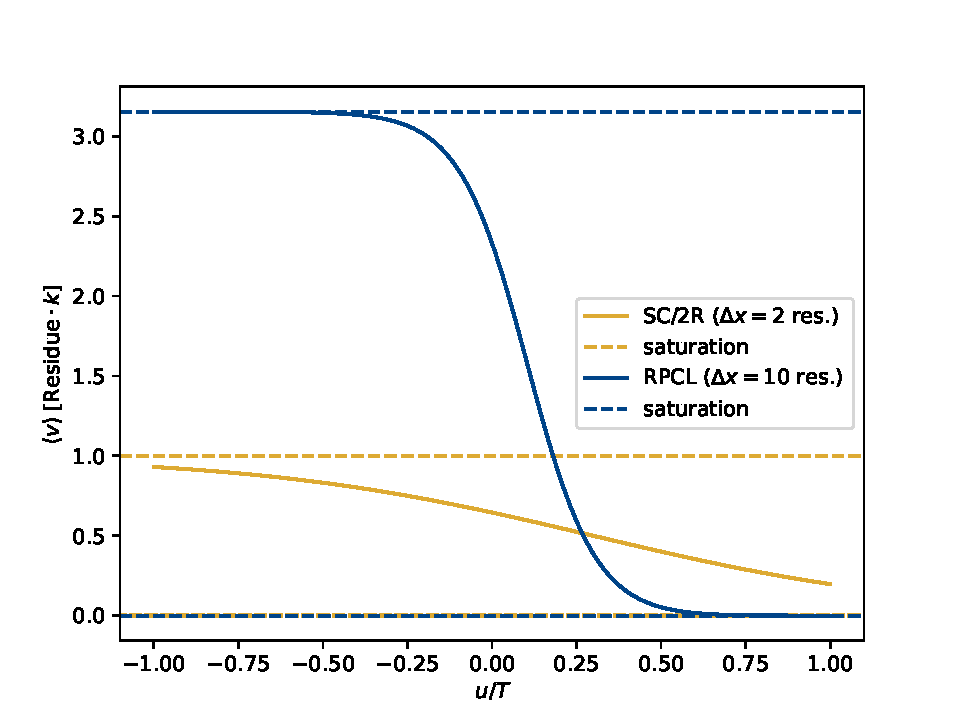
\includegraphics[width=\textwidth]{images/force.pdf}
        \caption{Average substrate translocation velocity as a function of the potential energy for a unit residue translocation over temperature for SC/2R (yellow) and RPCL (blue) models. The potential is generated by a constant force opposing the AAA+ ATPase substrate translocation.}
        \label{fig:force}
    \end{figure}
    
    The second important feature visible in Fig.~\ref{fig:force} is the sigmoidal shape of the average velocity, inversely related to the force. The inverse relation comes from the fact that the force acts as a barrier that the ATPase has to overcome to translocate the substrate and similarly facilitates its translocation in the reverse direction. The saturation comes from the fact that for extreme forces, the reactions associated with a translocation favored by the force in the kinetic scheme have an exponentially big rate so that when the system is in the initial state of the reaction, it will almost instantaneously jump to the resulting state, and similarly, the rate of reactions disfavored by the force is exponentially small so that this reaction is practically never realized. Therefore, the probability flux in the loop in essentially determined by the other reactions.
    
    This result was predictable when looking at the analytical expression of the steady-state probabilities and the average velocity. We illustrate this with the SC/2R model, but it would be similar for RPCL since both models are made of a single loop. Consider a large force intensity that will inhibit the forward translocation of the substrate. Mathematically, this corresponds to the situation $u \rightarrow \infty$, and thus the rates $k_\uparrow \rightarrow 0$ and $k_\downarrow \rightarrow\infty$ while all the other rates are left unchanged. In this limit, the steady-state probabilities Eq.~\eqref{eq:sc2r-steady-state-probabilities} become:
    \begin{equation}
    \begin{split}
        p_A &\propto k_s k_{DT} + k_\downarrow k_s + k_\uparrow k_{DT} 
            \approx k_\downarrow k_s \\
        p_B &\propto k_h k_\downarrow + k_{DT} k_h + k_{TD} k_\downarrow 
            \approx k_\downarrow (k_h + k_{TD}) \\
        p_C &\propto k_\uparrow k_{TD} + k_s k_{TD} + k_h k_\uparrow
            \approx 0
    \end{split}
    \end{equation}
    since $k_\downarrow$ appears in the denominator but not in the numerator of $p_C$, shrinking it to zero. In this limit, $k_\downarrow$ factorizes in $p_A$ and $p_B$, and thus are canceled out by the normalization constant. Therefore, the probabilities are:
    \begin{equation}
    \begin{split}
        p_A &= \frac{k_s}{k_s + k_h + k_{TD}} \\
        p_B &= \frac{k_h + k_{TD}}{k_s + k_h + k_{TD}}
    \end{split}
    \end{equation}
    The interpretation is that in this limit, the upward protomer translocation $k_\uparrow$ and state $C$ are removed from the kinetic scheme, and a reaction $A\to B$, an $\text{ATP}\to\text{ADP}$ exchange followed immediately by a downward protomer translocation (with rate canceled out), with an effective rate $k_{TD}$ is added. Then state $A$ can only be reached from state $B$ with rate $k_s$, and state $B$ can be reached from $A$ either by hydrolysis with rate $k_h$ or by the newly added effective reaction with rate $k_{TD}$. Consequently, the average velocity Eq.~\eqref{eq:sc2r-average-velocity} becomes:
    \begin{equation}
        \left\langle v \right\rangle \propto - \Delta x k_s k_{TD}
    \end{equation}
    We see in particular that even though in Fig.~\ref{fig:force} the average velocity seems to fall to zero for large forces, it actually saturates to a non-null but negative value. The speed is close to zero since the value of $k_{DT} \sim 1$, [ATP]/[ADP] $\gg 1$ and then $k_{TD}$ being fixed by Eq.~\eqref{eq:kdt-ktd-ratio} results in a very small value.
    
    The same reasoning can also be applied to the other limit $u\rightarrow -\infty$ and to the RPCL model. For the sake of completeness, all the saturated velocities are summarized here:
    \begin{equation}
    \begin{split}
        \left\langle v \right\rangle_{SC/2R} &=
            \begin{cases}
                \Delta x \frac{k_h k_{DT}}{k_h + k_{DT} + k_{TD}},
                    & \text{for } u\rightarrow -\infty \\
                - \Delta x \frac{k_s k_{TD}}{k_s + k_h + k_{TD}},
                    & \text{for } u\rightarrow \infty
            \end{cases} \\
        \left\langle v \right\rangle_{RPCL} &= 
            \begin{cases}
                \Delta x \frac{\bar{k}_h k_{DT} k_{\uparrow cont.}}{k_{DT} k_{\uparrow cont.} + k_{TD} \bar{k}_{\downarrow ext.} + \bar{k}_h k_{TD} + \bar{k}_h k_{\uparrow cont.} + k_{DT} \bar{k}_{\downarrow ext.} + \bar{k}_h k_{DT}}, 
                    & \text{for } u\rightarrow -\infty \\
                - \Delta x \frac{k_s k_{TD} \bar{k}_{\downarrow ext.}}{k_s k_{\uparrow cont.} + k_s k_{TD} + \bar{k}_h k_{TD} + \bar{k}_h k_{\uparrow cont.} + k_{TD} \bar{k}_{\downarrow ext.} + k_s \bar{k}_{\downarrow ext.}},
                    & \text{for } u\rightarrow \infty
            \end{cases}
    \end{split}
    \end{equation}
    and these analytical expressions are represented in dashed lines in Fig~\ref{fig:force}, which shows that the derivation above is consistent with the numerical implementation.
    
    We remember that in the RPCL model, we arbitrarily considered a substrate translocation during the upward extension ($k_{\uparrow ext.}$) and downward contraction ($k_{\downarrow cont.}$) of the ATPase and not during the upward contraction ($k_{\uparrow cont.}$) and downward extension ($k_{\downarrow ext.}$). One could choose instead to consider the translocation during the latter two reactions, or even split it, half the translocation during the former two reactions and half during the latter two reactions. This would not change the qualitative results highlighted here.

\subsection{Defective protomer}
    The last experiment we conduct studies how AAA+ ATPase dynamics are affected when a protomer is defective and hydrolyzes at a reduced rate. All the other characteristics of the defective protomers, in particular the spontaneous synthesis rate, stay unchanged, as well as all the other defectless protomers. 

    The undistinguishability assumption we made when introducing the models no longer holds. For the RPCL model, we consider two loops linked at the fully-ATP-bound-flat configuration, with one loop representing the reaction sequence of the defective protomer and the second loop being the reaction sequence of any $N-1$ defectless protomer, merged into a single loop, similarly as we did in the original model, since in this particular state, any protomer can randomly hydrolyze its ATP molecule. For the SC/2R model, we have no choice but to implement a large loop with the reaction sequence of each protomer consecutively. The defective protomer has a reduced hydrolysis rate $k_h\mapsto \alpha k_h$, where $\alpha$ is the defect factor.

    We show in Fig.~\ref{fig:defective} the effect of this defective protomer on the two models SC/2R and RPCL. With a defect factor $\alpha = 0.1$, SC/2R's average velocity is visibly reduced, both empirically and analytically, in a consistent manner. Compared to the defectless case, we see that the time between translocation events is more irregular, with longer plateaux, which is supported by the heavier-tail on the sojourn times histogram. This is because in this model, when the defective protomer is in the lowest position, there is no other path for the cycle to continue than to wait for it to hydrolyze its ATP molecule, and due to the defect factor, this waiting time is longer. On the other hand, with RPCL, the presence of a defective protomer affects substantially less the average velocity, as we can see on the trajectory and the sojourn times histogram. This is explained by the fact that in this model, the dynamics never depend on the defective protomer to hydrolyze its ATP molecule to continue because all protomers compete in parallel to hydrolyze their ATP molecule, and the only effect is that the defective protomer is less likely to be the first one to do so. Even in the limit $\alpha\rightarrow 0$, it would stay almost unaffected by the defect, whereas, in the SC/2R model, the ATPase would stop entirely. This result is consistent with experimental data where it has been shown that the ATPase is not significantly affected when the hydrolysis rate of a protomer is diminished\cite{desantis_operational_2012}.

    \begin{figure}[h]
        \hspace*{-0.25\textwidth}
        \centering
        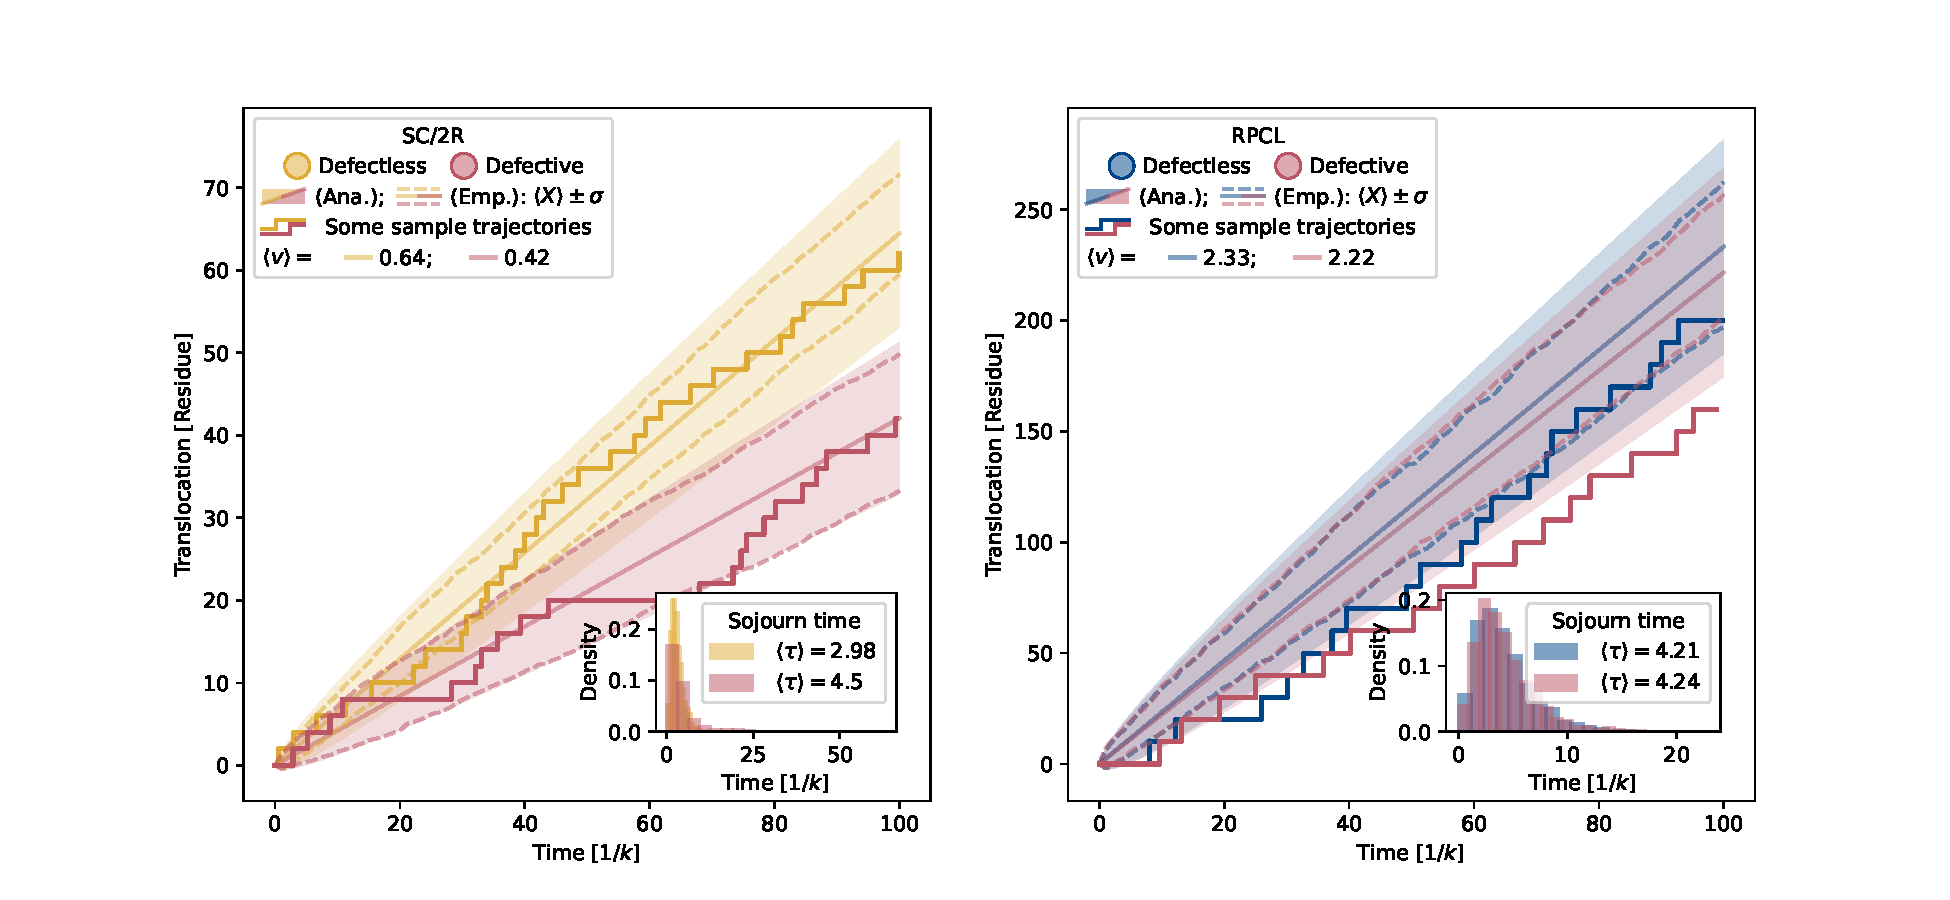
\includegraphics[width=1.5\textwidth]{images/defective.pdf}
        \caption{Comparison of the effects of a defective (red) protomer with hydrolysis rate ten times smaller on the dynamics of SC/2R (yellow) and RPCL (blue) models. Colored solid lines are trajectories, grey solid line and pale areas are analytical expected substrate translocation and standard deviation, dashed lines are empirical standard deviation. Average velocity in defectless and defective cases and the distribution of sojourn times between translocation events are computed. Physical rates are chosen to maintain ATPase activity.}
        \label{fig:defective}
    \end{figure}


\section{Conclusion}
\label{sec:conclusion}
In this work, we have studied two models of the mechanism of action of AAA+ ATPase, the Sequential Clockwise/2-Residue Step (SC/2R) model based on structural biology data and its analysis made by Shorter J. et al.\cite{shorter_spiraling_2019}, and our alternative model, the Random Protomer Concertina Locomotion (RPCL) model based on physical assumptions about the nature of the interaction potential between two neighboring protomers and the resulting minimal energy configuration of the ATPase, which are a flat and a staircase-like configurations, both having been observed experimentally\cite{shorter_spiraling_2019}. To conduct our study, we have implemented the two models in the kinetic scheme framework, which was first introduced in detail. The idealized models are both made of a single loop. Still, the key difference resides in the fact that in the SC/2R model, each protomer consecutively undergoes a hydrolysis-translocation-exchange reaction sequence. In contrast, in the RPCL model, all protomers compete in parallel to hydrolyze their ATP molecule, and the first one to do so induces the substrate translocation. Using simulations and analytical calculations, we analyzed the dynamics of the ATPase from the perspective of both models, focusing on the average velocity and the ATP consumption rate.

Comparing sample trajectories of the two models, we have shown that at equal average velocity, RPCL consumes five times less ATP and has a translocation steplength five times longer than SC/2R by moving steps five times longer, which better matches experimental data\cite{avellaneda_processive_2020}. We have also studied the response of the ATPase to an external pulling force opposing the substrate translocation. We have shown that for both models it results in a sigmoidal shape of the average velocity inversely related to the force, which is can be explained using the analytical solution of the kinetic scheme, but was not the expected result looking at experimental data which instead predicts a threshold force intensity under which the velocity is not significantly affected and over which the velocity drastically falls. However, the measurements were subject to high uncertainties and should be investigated further\cite{avellaneda_processive_2020}. Finally, we have studied the effect of a defective protomer on the dynamics of the ATPase, and we have shown that when one protomer has a reduced hydrolysis rate, the average velocity is visibly reduced for the SC/2R model, whereas it is almost unaffected for the RPCL model, which is consistent with experimental data\cite{desantis_operational_2012}.

In light of these results, we argue that the RPCL model should be favored over the SC/2R model, as its simulated trajectories and dynamics better reproduce experimental data. The predicted existence of a flat configuration, the larger translocation stepsize and the behavior in case of a defective protomer are three key points that enable us to discriminate the two models. 

We believe that the RPCL model is a good starting point to understand the dynamics of the ATPase, but it is still a very idealized model, raising numerous questions. Here we list some of them:
\begin{itemize}
    \item What is the nature of the interaction potential between two neighboring protomers, and is the linear approximation appropriate? If not, does the new potential energy landscape results in the same minimal energy configurations?
    \item How is post-hydrolysis protomer modified on a structural level to alter the interaction potential with its neighbor?
    \item Why are some protomers fixed to the substrate during the extension and contraction while some others are not?
    \item Are there other configurations observed experimentally, and how can we extend the RPCL model to encompass them?
    \item The extension and contraction are modeled as occurring abruptly after a sojourn time sampled from an exponential distribution. What is the physics underlying these reactions, and is this simplification appropriate?
    \item This idealized model only considers states belonging to the main loop, where at most one protomer is in ADP-bound state. We only skimmed over the possibility of leaving this main loop by adding a single \emph{out} state reachable from any state. Should one consider a more complex model with more states?
\end{itemize}

Science is an iterative process where empirical, numerical, and theoretical advances are poetically complementary, and this work paved the way for future research on the dynamics of AAA+ ATPases. Moving forward, the next step would be to compare the RPCL model with various experimental setups in order to refine the model or even discard it in favor of a better one. Other alternative models have been proposed\cite{lin_aaa+_2022}, and it would be interesting to translate them into the kinetic scheme framework to see how they compare with the RPCL model. Experiments would also help to fine-tune all the degrees of freedom of the model, namely all the rates; even though the qualitative results are not expected to change, we should not be too confident; interesting physics can lie where we least expect it. 


\section*{Acknowledgments}
    I want to thank my advisor, Pr. De Los Rios, for his guidance and support throughout this project, his trust in my independent work, and his compassion in difficult personal situations. I'd also like to thank my sister, Aude, to whom I dedicate this work and with whom I've spent the best years of my studies and my life so far. Her advice throughout my academic and personal life has been invaluable, and I am grateful for her support and love. I wish her the best for her future, academic or otherwise; only time will tell. It is with a lot of emotion that I conclude this work and my studies, and I hope it will be the beginning of a new chapter in my life.

\printbibliography

\appendix

\section{Master equation derivation}
\label{app:master-equation}
    The master equations are the differential equations that govern the evolution of the probability distribution $p_i(t)$ of being in state $i$ at a given time $t$. Let's derive it partially rigorously.

    Let $S(t)$ be the random variable representing the system's state at time $t$. There are $N$ discrete states denoted by the letters $i,j,k$. The set of predecessors and successors of state $i$ are denoted by $R_i^-$ and $R_i^+$, respectively. The transition rates from state $i$ to state $j$ are denoted by $k_{ij}$. The transition rates are non-negative, and we use the convention that $k_{ij}=0$ if $j\notin R_i^+$, $k_{ij}=0$ if $i\notin R_j^-$, and $k_{ii}=0$ for all $i=1,2,\dots,N$.
    
    First, consider a single reaction $i\to j$. We associate to this reaction a random variable $T_{ij}$ denoting the time it takes for the reaction to occur. Since the reaction follows an exponential distribution, we have the following:
    \begin{equation}    
        \mathbb{P}(T_{ij}<t) = 1-\exp(-k_{ij}t)
    \end{equation}
    
    Then, suppose we are in state $i$, and let's study the passage from this state to a chosen successor $j^*\in R_i^+$. Consider the event $\left<i\xrightarrow{\Delta t}j^*\right> :=$ \textit{the system has jumped from $i$ to $j^*$ at some time in the interval $[t,t+\Delta t]$}. This event is equivalent to the event $\{(T_{ij^*}<\Delta t) \wedge (\forall j\neq j^*, T_{ij}>\Delta t)\}$. Since the reactions are independent, the joint probability of the reaction times splits into the product of the individual probabilities. Therefore, the probability of the abovementioned event is given by:
    \begin{equation}
    \begin{split}
        &\mathbb{P}\left((T_{ij^*}<\Delta t) \wedge (\forall j\neq j^*, T_{ij}>\Delta t)\right) \\
        &= \mathbb{P}(T_{ij^*}<\Delta t)\prod_{j\neq j^*}\mathbb{P}(T_{ij}>\Delta t) \\
        &= (1-\exp(-k_{ij^*}\Delta t))\exp(-\sum_{j\neq j^*}k_{ij}\Delta t) \\
        &= (1 - (1 - k_{ij^*}\Delta t + o(\Delta t)))(1 - \sum_{j\neq j^*}k_{ij}\Delta t + o(\Delta t)) \\
        &= k_{ij^*}\Delta t + o(\Delta t)
    \end{split}
    \end{equation}
    where we used the 1st-order Taylor expansion of the exponential function. 
    
    Moreover, the event $\left<i\xrightarrow{\Delta t}i\right>:=$ \textit{the system stayed in state $i$ during a time interval of length $\Delta t$} has probability:
    \begin{equation}
    \begin{split}
        &\mathbb{P}(\forall j\in R_i^+, T_{ij}>\Delta t) 
        = \prod_{j\in R_i^+}\mathbb{P}(T_{ij}>\Delta t) 
        = e^{-\sum_{j\in R_i^+}k_{ij}\Delta t} \\
        &= 1 - \sum_{j\in R_i^+}k_{ij}\Delta t + o(\Delta t)
    \end{split}
    \end{equation}
    
    Finally, we derive the desired master equation. To be in state $j^*$ at time $t+\Delta t$, there are logically only two possibilities: either the system was already in state $j^*$ at time $t$ and did not jump to any other state in the interval $[t,t+\Delta t]$, or the system was in another state $i\in R_{j^*}^-$ at time $t$ and jumped to $j^*$ in the interval $[t,t+\Delta t]$. We control the size of the interval $\Delta t$ such that maximum one reaction can occur during the interval $[t,t+\Delta t]$. The jump probabilities at a given time are difficult to compute, but what the conditional jump probability \emph{given} that we start in a given state $i$ at time $t$, namely $\left<i\xrightarrow{\Delta t} j\right>$ are known. Therefore, we can write the probability of being in state $j^*$ at time $t+\Delta t$ as:
    \begin{equation}
    \begin{split}
        &\mathbb{P}(S(t+\Delta t)=j^*) \\
        &= \mathbb{P}(S(t)=j^*)\mathbb{P}(\left<j^*\xrightarrow{\Delta t}j^*\right>) + \sum_{i\in R_{j^*}^-}\mathbb{P}(S(t)=i)\mathbb{P}(\left<i\xrightarrow{\Delta t}j^*\right>) \\
        &= \mathbb{P}(S(t)=j^*)(1 - \sum_{k\in R_{j^*}^+}k_{j^*k}\Delta t) + \sum_{i\in R_{j^*}^-}\mathbb{P}(S(t)=i)(k_{ij^*}\Delta t) + o(\Delta t)
    \end{split}
    \end{equation}
    
    Reordering the terms, we find
    \begin{multline}
        \frac{\mathbb{P}(S(t+\Delta t)=j^*) - \mathbb{P}(S(t)=j^*)}{\Delta t} \\
        = \sum_{i\in R_{j^*}^-}\mathbb{P}(S(t)=i)k_{ij^*} - \mathbb{P}(S(t)=j^*)\sum_{k\in R_{j^*}^+}k_{j^*k} + \frac{o(\Delta t)}{\Delta t}
    \end{multline}
    
    Taking the limit $\Delta t\to 0$, we find the master equation
    \begin{equation}
        \frac{d\mathbb{P}(S(t)=j^*)}{dt} = \sum_{i\in R_{j^*}^-}\mathbb{P}(S(t)=i)k_{ij^*} - \mathbb{P}(S(t)=j^*)\sum_{k\in R_{j^*}^+}k_{j^*k}
    \end{equation}
    
    Applying the same reasoning to all states $j^*=1,2,\dots,N$, changing the dummy indices, using the convention $k_{ij}=0$ when states $i$ and $j$ are not connected, and using the notation $p_i(t) = \mathbb{P}(S(t)=i)$, we find the $N$ coupled differential equations
    \begin{equation}
        \dot{p}_i(t) = \sum_{j\in R_i^-}p_j(t)k_{ji} - p_i(t)\sum_{j\in R_i^+}k_{ij} = \sum_{j=1}^N \left(p_j(t)k_{ji} - p_i(t)k_{ij}\right)
    \end{equation}

\section{Existence and uniqueness of the steady-state distribution}
\label{app:steady-state-dist}
    Consider a system represented by its $N$-dimensional master equation $\dot{\mathbf{p}}(t) = \mathbf{M}\mathbf{p}(t)$, where $\mathbf{p}(t)$ is the column vector of components $p_i(t)$ and $\mathbf{M}$ is the matrix of components $M_{ij}=k_{ji} - \delta_{ij}\sum_{k=1}^N k_{ik}$, where $\delta_{ij}$ is the Kronecker delta. We assume that the corresponding kinetic scheme of the system is connected, and we use the convention $k_{ii}=0$.
    We show that the system has a unique steady-state distribution $\mathbf{p}^*$, i.e. a solution of the equation $\mathbf{M}\mathbf{p}^* = 0$.

    \begin{proposition}
        A solution of the continuous time system $\dot{\mathbf{p}}(t) = \mathbf{M}\mathbf{p}(t)$ is a steady-state if and only if it is a fixed-point of a discrete-time system $\mathbf{p}^{(t+1)} = \mathbf{W}\mathbf{p}^{(t)}$ with stochastic matrix $\mathbf{W} := \mathbf{I} + \Delta t \mathbf{M}$, where $\mathbf{I}$ is the identity matrix and $\Delta t := \frac{1}{N\max_{i,j}k_{ij}}$.
    \end{proposition}

    \begin{proof}
        \begin{equation}
            \underbrace{\mathbf{p} \overset{!}{=} \mathbf{W}\mathbf{p}}_\text{fixed-point} 
            = \mathbf{p} + \Delta t \mathbf{M}\mathbf{p}
            \iff \underbrace{\mathbf{M}\mathbf{p} = \mathbf{0}}_\text{steady-state}
        \end{equation}
    \end{proof}

    \begin{lemma}
        Any element of the stochastic matrix $\mathbf{W}$ is non-negative, and the sum of any column is 1.
    \end{lemma}
    
    \begin{proof} 
        \begin{multline}
            W_{ij} 
            = \delta_{ij} + M_{ij}\Delta t 
            = \delta_{ij} + (k_{ji} - \delta_{ij}\sum_{k=1}^N k_{ik})\Delta t \\
            = k_{ji}\Delta t + \delta_{ij} \left(N\max_{i,j}k_{ij} - \sum_{k=1}^N k_{ik}\right)\Delta t
            \geq 0
        \end{multline}
        and
        \begin{equation}
            \sum_{i=1}^N W_{ij}
            = 1 + \sum_{i=1}^N \left(k_{ji} - \delta_{ij}\sum_{k=1}^N k_{ik}\right) \Delta t
            = 1 + \left(\sum_{i=1}^N k_{ji} - \sum_{k=1}^N k_{jk}\right) \Delta t
            = 1
        \end{equation}
    \end{proof}

    \begin{proposition}
        There exists a fixed-point $\mathbf{p}^*$ of the discrete time system on the probability simplex $\Delta_N := \{\mathbf{p}\in\mathbb{R}^N \mid \sum_{i=1}^N p_i = 1 \wedge \forall i, p_i\geq 0\}$.
    \end{proposition}

    \begin{proof}
        First, $\mathbf{W}$ is an endomorphism $\mathbf{W}: \Delta_N \to \Delta_N$, since for $\mathbf{p}^{(t)}\in \Delta_N$, we have
        \begin{equation}
            p_i^{(t+1)} 
            = \left(\sum_{j=1}^N W_{ij}p_j^{(t)}\right) 
            = \sum_{j=1}^N \underbrace{W_{ij}}_{\geq 0}  p_j^{(t)} 
            \geq 0
        \end{equation}
        and
        \begin{equation}
            \sum_{i=1}^N p_i^{(t+1)} 
            = \sum_{i=1}^N \left(\sum_{j=1}^N W_{ij}p_j^{(t)}\right) 
            = \sum_{j=1}^N \underbrace{\left(\sum_{i=1}^N W_{ij}\right)}_{=1}  p_j^{(t)} 
            = \sum_{j=1}^N p_j^{(t)} 
            = 1
        \end{equation}
    
        Moreover, $\mathbf{W}$ is linear and thus continuous, and $\Delta_N$ is a compact convex set. Therefore, the Brouwer fixed-point theorem implies the existence of a fixed-point, which we call $\mathbf{p}^*$.
    \end{proof}

    \begin{proposition}
    \label{prop:coordinates}
        The coordinates of the fixed point $\mathbf{p}^*\in \Delta_N$ are strictly within $]0, 1[$.
    \end{proposition}

    \begin{proof}
        If the kinetic scheme of the continuous-time system is connected, then so is the kinetic scheme of the discrete-time system. Therefore, by definition of connectivity, $(W^N)_{i,j}>0$, $\forall i,j$. Moreover, since $\mathbf{p}^*$ is a fixed-point, we have $\mathbf{p}^* = \mathbf{W^N}\mathbf{p}^*$. First, any coordinate is strictly positive:
        \begin{equation}
            p_i^* = \sum_{j=1}^N (W^N)_{i,j}p_j^* > 0 
        \end{equation}
        since it is a sum of non-negative terms, and at least one of them is strictly positive. On the other hand, if one coordinate is 1, all the others must be zero since the sum of the coordinates is 1, which contradicts the previous statement. Therefore, all the coordinates of $\mathbf{p}^*$ are strictly within $]0, 1[$.
    \end{proof}

    \begin{corollary}
    \label{cor:unique}
        The fixed-point $\mathbf{p}^*\in \mathring\Delta_N$ is unique on $\mathring\Delta_N$.
    \end{corollary}

    \begin{proof}
        Prop.~\ref{prop:coordinates} restricts the existence of a fixed-point on the boundary of the probability simplex $\Delta_N$. Now assume there exists another fixed-point $\mathbf{q}^*\in \mathring\Delta_N$, different from $\mathbf{p}^*$. By linearity, any linear combination of $\mathbf{p}^*$ and $\mathbf{q}^*$ is also a fixed-point of $\mathbf{W}$. Therefore, there must exists a linear combination $\mathbf{r}^* = \alpha(\mathbf{p}^* + \beta\mathbf{q}^*)$ that lies on an edge of the probability simplex ($\mathbf{p}^*$ and $\mathbf{q}^*$ differ on at least one coordinate, $p^*_i\neq q^*_i \neq 0$, choose $\beta = -\frac{p^*_i}{q^*_i}$ and choose $\alpha$ so that $\mathbf{r}^*$ is normalized), which contradicts Prop.~\ref{prop:coordinates}. 
    \end{proof}

    \begin{proposition}
    \label{prop:unique}
        The fixed-point $\mathbf{p}^*\in \mathring\Delta_N$ is unique (up to a constant) on $\mathbb{R}^N$.
    \end{proposition}

    \begin{proof}
        The proof is similar to Cor.~\ref{cor:unique}. Assume there exists a fixed-point $\mathbf{q}^*$ in a different orthant than the probability simplex. Then, construct the linear combination $\mathbf{r}^* = \alpha(\mathbf{p}^* + \beta\mathbf{q}^*)$ that lies on the boundary of the probability simplex ($\mathbf{p}^*$ and $\mathbf{q}^*$ differ on at least one nonzero coordinate, $p^*_i\neq q^*_i \neq 0$, choose $\beta = -\frac{p^*_i}{q^*_i}$ and choose $\alpha$ so that $\mathbf{r}^*$ is normalized), which contradicts Prop.~\ref{prop:coordinates}.
    \end{proof}

    \begin{theorem}
        The fixed-point $\mathbf{p}^*\in \Delta_N$ is the unique steady-state distribution of the continuous-time system $\dot{\mathbf{p}}(t) = \mathbf{M}\mathbf{p}(t)$.
    \end{theorem}
    
    \begin{proof}
        Prop.~\ref{prop:unique} says that the subspace of fixed-points of $\mathbf{W}$ has dimension 1. The relation between $\mathbf{W}$ and $\mathbf{M}$ immediately implies that the kernel of the latter is also of dimension 1. Therefore, the linear system $\mathbf{M}\mathbf{p}^* = \mathbf{0}$ has a unique solution (up to a constant). The steady-state $\mathbf{p}^*$ is the positive and normalized solution.
    \end{proof}

    \begin{remark}
        To show the global convergence property of the steady-state distribution, one has to use the Liapunov function presented in \cite{schnakenberg_network_1976}.
    \end{remark}

\section{Non-ideal models, presence of an \emph{out} state}
\label{app:non-ideal-model}
In the idealized models we introduced in Secs.~\ref{subsec:sc2r-model}~and~\ref{subsec:rpcl-model}, we considered that the ATPase is always in one of the $N$ states of the \emph{main loop}. To alleviate this assumption, we add a single \emph{out} state connected to every state of the main loop, representing any state not considered in the ideal model. This could be, for example, a situation where a second protomer hydrolyzes or exchanges its ATP, which are situations not currently considered in the main loop. Adding this state to the kinetic scheme introduces new thermodynamic loop laws, which result in $N-1$ independent constraints on the rates. To simplify, we consider that the rate from the \emph{out} state to any state of the main loop is the same, and we denote it by $k_{in}$. It remains to fix the out rate $k_{out}$ from an arbitrary main loop state, and then all the other out rates are constrained by loop laws.

In Fig.~\ref{fig:non-ideal}, we show that, as one would expect, the time spent in the main loop, measured by the summed steady-state probabilities of the main loop states, diminishes as $k_{out}$ increases.

\begin{figure}[h]
    \centering
    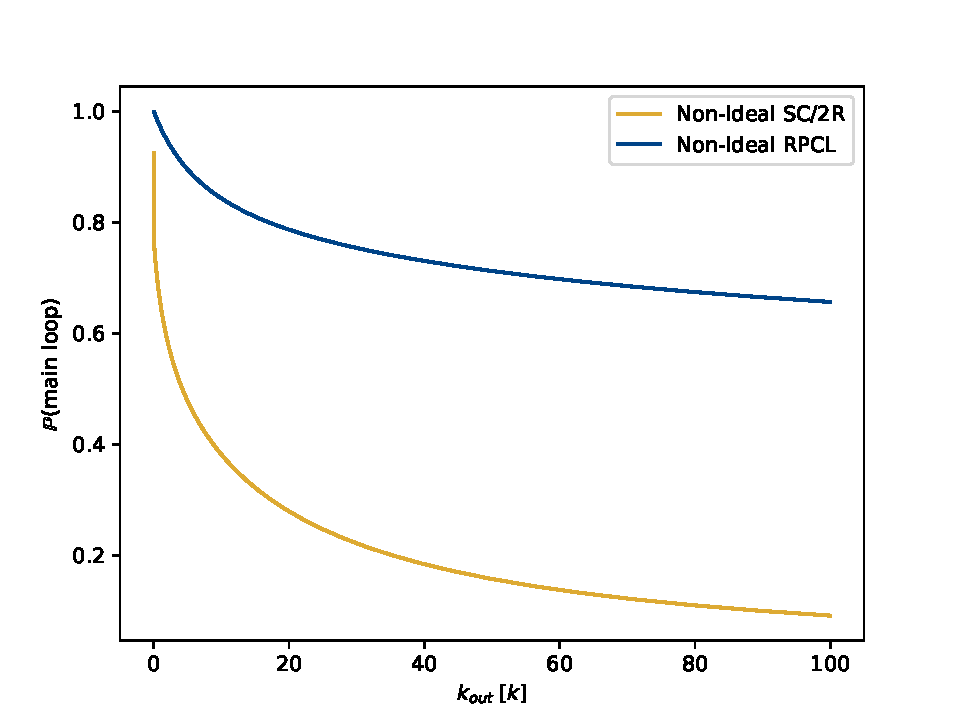
\includegraphics[width=0.8\textwidth]{images/non_ideal.pdf}
    \caption{Effect of adding an \emph{out} state to the ideal models representing any other state. The probability of being in a state belonging to the ideal SC/2R (yellow) and RPCL (blue) models as a function of the exit rate to the \emph{out} state is shown.}
    \label{fig:non-ideal}
\end{figure}

\section{Relation between average velocity and [ATP]/[ADP]}
\label{app:average-velocity-vs-atp-adp-ratio}
Here, we confirm numerically the analytical prediction in Eqs.~\eqref{eq:sc2r-average-velocity}~and~\eqref{eq:rpcl-quantities-of-interest} that average velocity for both SC/2R and RPCL models is positively related with the deviation of [ATP]/[ADP] concentration ratio from its equilibrium value, with a proportional relation in the limit of small deviation, and saturation in the limit of large deviation. We show in Fig.~\ref{fig:velocity-vs-atp-adp-ratio} the average velocity as a function of the ratio [ATP]/[ADP] over its equilibrium value for both models. We see that the average velocity matches the described behavior. The reason for saturation is similar to the one for the force-velocity relation in Sec.~\ref{subsec:force}. In a nutshell, the reaction affected by the value of [ATP]/[ADP] becomes so favored that it can be effectively removed, and then the flux on the loop of the kinetic scheme is limited by the other reactions.

\begin{figure}[h]
    \centering
    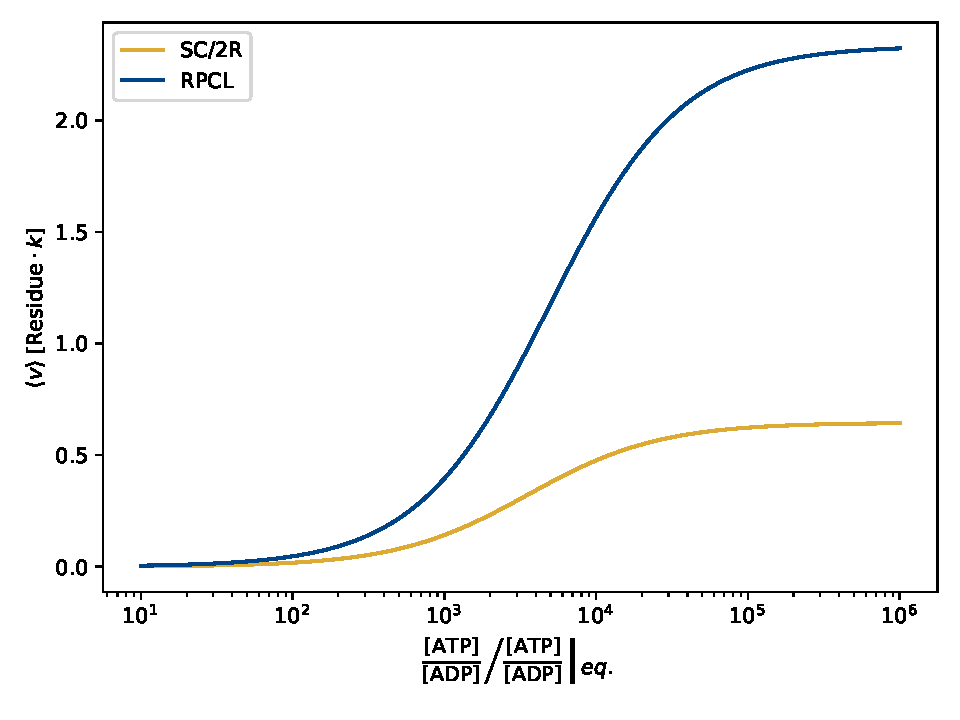
\includegraphics[width=0.8\textwidth]{images/velocity_vs_atp_adp_ratio.pdf}
    \caption{Variation of the average translocation velocity of SC/2R (yellow) and RPCL (blue) models when the [ATP]/[ADP] concentration ratio deviates from its equilibrium value.}
    \label{fig:velocity-vs-atp-adp-ratio}
\end{figure}


\end{document}
